\chapter{Literature Review}
\section{Introduction}
This section aims to summarise the current body of knowledge available on the topic. 
The relevance to this information and the report will also be indicated. 
%after this section the reader will understand every term, idea and concept that existed prior to the undertaking of the project.
	\section{K- value}
	The current K-values used for the design of timber elements are taken from the EURO code (ref TODO \citep{Euro:2004})  
	\begin{figure}[H]
	\label{kvalue_fig}
	\centering
	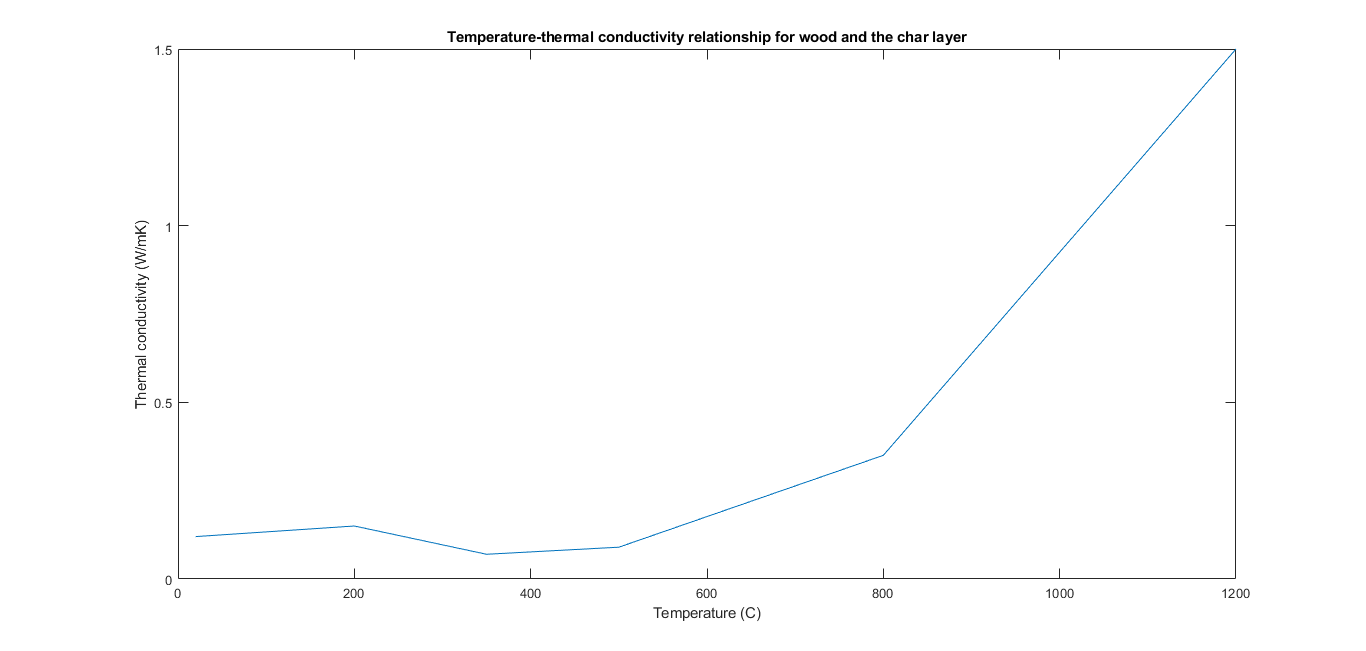
\includegraphics[width = \linewidth]{kvalues_euro.png}
	\end{figure}
	
	\section{Bayes' theorem of inverse problems}
%	Statistical and Computational Inverse problems by Kaipio and Somersalo Chapter 3
% 	The Bayesian approach to Inverse Problems Dashti and Stuart
	The method of statistical inversion is dependant on a fundamental understanding of the Bayes' theorem of inverse problems. 
	The student obtained this understanding through studying Chapter 3 of Statistical and Computational Inverse problems by \citet{Kaipo:2005}, further referred to merely as Kaipio. 
	There are four principles of Statistical inversion that is essential to the thorough understanding of these models. 
	Firstly it is the principle that any variable in the model needs to be modelled as a random variable. 
	This randomness is based on the extent of information that is available. 
	To ensure that the extent of knowledge is accurately portrayed in the model the extent of knowledge will be coded into the probability distributions assigned to the different variables. 
	Finally it needs to be understood that the solution of a statistical inversion is a posterior probability distribution.
	A generalized equation of Bayes' theorem can be seen in \ref{bayes_eq} taken from Kaipo. 
	
	\begin{equation}
	\label{bayes_eq}
	\pi_{\text{post}}(x) = \pi(x|y_{\text{observed}}) = \frac{\pi_{\text{pr}}(x) \pi(y_{\text{observed}}|x)}{\pi (y_{\text{observed}})}	
	\end{equation}
	
	\section{Heat diffusion equation}
	In it's simplest form the one dimensional heat diffusion equation is a partial differential equation \ref{heat_eq} dependant on the temperature and thickness of the element. 
	The heat diffusion equation is based on Fourier's Law
	
	
	\begin{equation}
	\label{heat_eq}
		q = -k \frac{dT}{dx}
	\end{equation}